\documentclass{article}
\usepackage{graphicx}
\usepackage{amsmath}
\usepackage{amsfonts} 
% or 
\usepackage{amssymb}

\usepackage{tikz}
\usepackage{pgfplots}
 
\pgfplotsset{compat = newest}
\usepackage{cancel}
\usepackage[margin=1in]{geometry}

\begin{document}

\title{A-Level Maths Notes}
\maketitle

\section{Laws of Indices}

\subsection{Subsets of Real Numbers}

\subsubsection{Natural Numbers}
Natural Numbers are positive whole numbers. Weather or not Zero is natural
is disputed but the exam boards say it isn't. They are the "Counting Numbers"
 and are represented by the following:

\begin{equation}
    \label{simple_equation}
    \mathbb{N}_0 = \{0, 1, 2, \dots\}
\end{equation}

\begin{equation}
	\label{simple_equation}
    \mathbb{N}_1 = \{1, 2, 3, \dots\}
\end{equation}

\subsubsection{Integers}
Integers are whole numbers. They can be positive or negative  and are represented by the following:

\begin{equation}
    \label{simple_equation}
    \mathbb{Z} = \{\dots, -3, -2, -1, 0, 1, 2, 3, \dots\}
\end{equation}

\subsubsection{Rational Numbers}
Rational Numbers are any real number that can be represented by a fraction. They are represented by the following:

\begin{equation}
	\label{simple_equation}
	\mathbb{Q} = \{ x | x = \frac{a}{b}, a,b \in \mathbb{Z} \text{ and } b \ne 0 \}
\end{equation}

\subsubsection{Real Numbers}
A real number is any number that is not complex or imaginary. They are represented by the following:

\begin{equation}
	\label{simple_equation}
	\mathbb{R} = \{x | -\infty <  x <\infty\}
\end{equation}

\begin{equation}
	\label{simple_equation}
	\mathbb{N} \subset \mathbb{Z} \subset \mathbb{Q} \subset \mathbb{R}
\end{equation}

\break
\subsection{Indices: The Laws of Indices}

\subsection{Multiplying Indices}
When multiplying indicies the following is true:
\begin{equation}
	\label{simple_equation}
	x^{p} \times x^{q} = x^{p + q}
\end{equation}
This reason for this becomes clear when we expand the expressions.
\\
For example:
\begin{gather*}
	x^2 \times x^3 = x^5\\
	\underbrace{
		\overbrace{x \times x}^{x^2} \times
		\overbrace{x \times x \times x}^{x^3}
	}_{x^5}
\end{gather*}

\subsubsection{Powers of Indices}

\begin{equation}
	\label{simple_equation}
	x^{pq} = (x^{p})^{q} = (x^{q})^{p} 
\end{equation}
The reason for this becomes clear when we expand the expressions.
\\
For example:

\begin{gather*}
	(x^2)^3 = x^6\\
	\underbrace{
		\overbrace{x \times x}^{x^2} \times
		\overbrace{x \times x}^{x^2} \times
		\overbrace{x \times x}^{x^2}
	}_{x^6}
\end{gather*}
\subsubsection{Division}

\begin{equation}
	\label{simple_equation}
	x^{p - q} = \frac{x^{p}}{x^{q}}
\end{equation}
The reason for this becomes clear when we expand the expressions.
\\
For example:

\begin{gather*}
	\frac{x^3}{x^2} = x^1\\
	\frac{\overbrace{x \times x \times x}^{x^3}}{\underbrace{x \times x}_{x^2}} =
	\frac{\overbrace{\cancel{x} \times \cancel{x} \times x}^{x^3}}{\underbrace{\cancel{x} \times \cancel{x}}_{x^2}} =
	x
\end{gather*}
\subsubsection{Rational Exponents}
Any rational exponent can be expressed as a power and a root:
\begin{equation}
	\label{simple_equation}
	\sqrt[q]{x}^{p} = x^{\frac{p}{q}}
\end{equation}


\begin{equation}
	\label{simple_equation}
	\sqrt[p]{x} = x^{\frac{1}{p}}
\end{equation}

\subsubsection{Zero}
Anything with a power of $0$ is always $1$ even in the case of $0$.
\begin{equation}
	\label{simple_equation}
	x^0 = 1
\end{equation}
This is true because you can always add a $\times 1$ as shown below:
\begin{equation}
	x^0 = 1 \times x^0 = 1 \times \cancel{x^0} = 1
\end{equation}

\subsubsection{Negative Exponents}
Negative exponents are defined as the following, this means that a larger magnitude of $p$ when $x>1$
will result in the expression evaluating to a smaller number.
\begin{equation}
	\label{simple_equation}
	x^{-p} = \frac{1}{x^p}
\end{equation}

\subsubsection{Reciprical}
The reciprocal is a special case of a negative exponent where the exponent is always $-1$.
\begin{equation}
	\label{simple_equation}
	x^{-1} = \frac{1}{x}
\end{equation}

\break
\section{Quadratic Functions and Graphs}

\subsection{Factorising Quadratics}

\subsubsection{Difference of Two Squares}
The difference of two squares is a rule that can help us
factorise quadratics in the form $ax^2 + b$ by using the
following identity:

\begin{equation}
	(a - b)(a + b) = a^2 + b^2
\end{equation}
The proof of this is fairly straight forward; we simply expand and simplify $(a - b)(a + b)$ to get $a^2 + b^2$.
\\
We can apply this identity when given a quadratic in the form $ax^2 + c$.

\begin{align*}
	&\text{First we rearrange to fit the identity}\\
	&(x\sqrt{a})^2 + \sqrt{c}^2\\
	&\text{Then we use the identity to split the expression into factors}\\
	&(x\sqrt{a} - \sqrt{c})(x\sqrt{a} + \sqrt{c})
\end{align*}
For example, we can factorise the quadratic $25x^2 - 16$:

\begin{align*}
	&\text{First we rearrange to fit the identity}\\
	&(x\sqrt{25})^2 - \sqrt{16}^2 = (5x)^2 - 4^2\\
	&\text{Then we use the identity to split the expression into factors}\\
	&(5x - 4)(5x + 4)
\end{align*}

\subsubsection{Factorising Quadratics in the form $x^2 + bx + c$}
In order to factorise a quadratic in the form $x^2 + bx + c$,
we need to find two numbers, $e$ and $f$ where $e + f = b$ and
$e \times f = c$ then sub them into the following expression:
\begin{equation}
	(x + e)(x + f)
\end{equation}
\\
For example, if given the quadratic $x^2 + 5x + 6$ we can factorise as shown by the following:
\begin{align*}
	2 \times 3 &= 6 \\
	2 + 3 &= 5 \\
	&\therefore \\
	x^2 + 5x + 6 &= (x + 2)(x + 3)
\end{align*}

\subsubsection{Factorising Quadratics in the form $ax^2 + bx + c$}
In order to factorise a quadratic in the form $ax^2 + bx +c$, we must first factor out $a$.
This gives us the following expression:
\begin{equation}
	a\left(x^2 + \frac{bx}{a} + \frac{c}{a} \right)
\end{equation}
\\
This makes it easy to factorise quadratics where both $b$ and $c$ are divisible by $a$
For Example, we can factorise the expression $2x^2 + 10x + 12$ with the following steps:

\begin{gather*}
	\text{We start by factoring out a}\\
	2\left(x^2 + \frac{10x}{2} + \frac{12}{2} \right) = 2(x^2 + 5x + 6)\\
	\text{We then factorise the new quadratic}\\
	2((x+2)(x+3)) = 2(x+2)(x+3)\\
	\text{Often our answer will be required in the form $(x + a)(x + b)$}\\
	(2x + 4)(x + 3) \text{ or } (x + 2)(2x + 6)
\end{gather*}
\\
However in some casees neither $b$ or $c$ are divisible by $a$.
For Example $16x^2 - 8x - 3$ though we can still use the same method.

\begin{gather*}
	16\left(x^2 - \frac{8}{16} - \frac{3}{16}\right)\\
	16\left(x + \frac{3}{4}\right)\left(x - \frac{1}{4}\right)
\end{gather*}
\subsection{Completing the Square}
Completing the square is act of rearranging a quadratic into the form $a(x + b)^2 +c$ to tell
us more information about the quadratic such as the turning point.

\subsubsection{Completing the Square for Quadratics in the form $x^2 + bx + c$}
For quadratics with a unit $x^2$ coefficient, we write our answer in the form \\
$(x+b)^2 + c$. To do this we use the steps show in the following example:
\\\\
We start with a quadratic:
\begin{equation}
	x^2 + 8x + 20
\end{equation}
We then half then make an expression in the form $(x+a)^2$ that
is equivalent to the same first two terms as the quadratic we started with
We do this by halving $b$ and putting it inside the brackets like so
\begin{equation}
	(x+4)^2 - 16= x^2 + 8x
\end{equation}
We then add a value on the end to make the starting quadratic
and the expression we ended up with equivalent
\begin{equation}
	(x + 4)^2 - 16 + 20 (x + 4)^2 - 16 + 20 
\end{equation}

\subsubsection{Completing the Square for Quadratics in the form $ax^2 + bx + c$}
For quadratics in with an $x^2$ coefficient that is not equal to $1$ it gets slightly more
complicated but the core idea stays the same.
\\\\
We start with a quadratic:
\begin{equation}
	2x^2 + 8x + 3
\end{equation}
We then factor out the $x^2$ coefficient like so:
\begin{equation}
	2(x^2 + 4x) + 3
\end{equation}
We then use the same method as previous this time remembering to multiply the number we move out of the parenthesis by $2$:
\begin{equation}	
	2(x + 2)^2 - 8 + 3 = 2(x + 2)^2 - 5
\end{equation}
\pagebreak
\subsection{Parabolas}

\subsubsection{Plotting Parabolas}
One way of plotting parabolas is to work out some specific points on the parabola and plot them.
\\
To do this we first start by calculating the y values for a given set of x values as shown below for
$y = x^2$:
\begin{center}
	\begin{tabular}{ | c | r | r | r | c | c | c | c | }
		\hline
		$x$ & $-3$ & $-2$ & $-1$ & $0$ & $1$ & $2$ & $3$\\ \hline
		$y=x^2$ &$9$ & $4$ & $1$ & $0$ & $1$ & $4$ & $9$\\
		\hline
	\end{tabular}
\end{center}
Once we have this data we can then plot it onto a graph such as the one below:
\begin{center}
	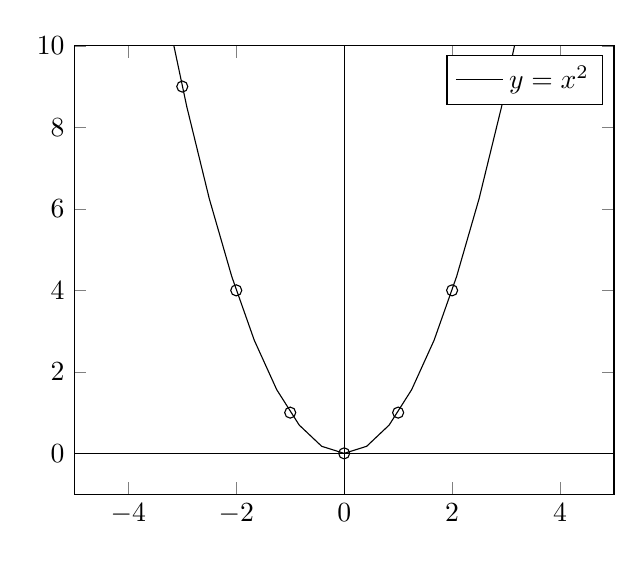
\begin{tikzpicture}
		\begin{axis}[
			xmin=-5, xmax=5,
    		ymin=-1, ymax=10,
		]
			\addplot[] {x^2};
			\addplot[only marks,mark=o] coordinates{(-3,9) (-2,4) (-1,1) (0,0) (1,1) (2,4) (3,9)};
			\legend{$y=x^2$}
			\draw[-] (-5,0)--(5,0);
			\draw[-] (0,-1)--(0,10);
		\end{axis}
	\end{tikzpicture}
\end{center}
\subsubsection{Sketching Parabolas from factorised quadratics}
In order to sketch a parabola, we need to know 3 points: Where on the parabola $x=0$ and 
where on the parabola $y=0$. We can do this by factorising. For example, the quadratic
$x^2 - x - 2$ can be factorised into $(x+1)(x-2)$. From there we can calculate the roots as
$(-1, 0)$ and $(2, 0)$ and the y intercept as $(0, -2)$. We can then roughly mark them on
some axis and then sketch a parabola that passes through those points.

\begin{center}
	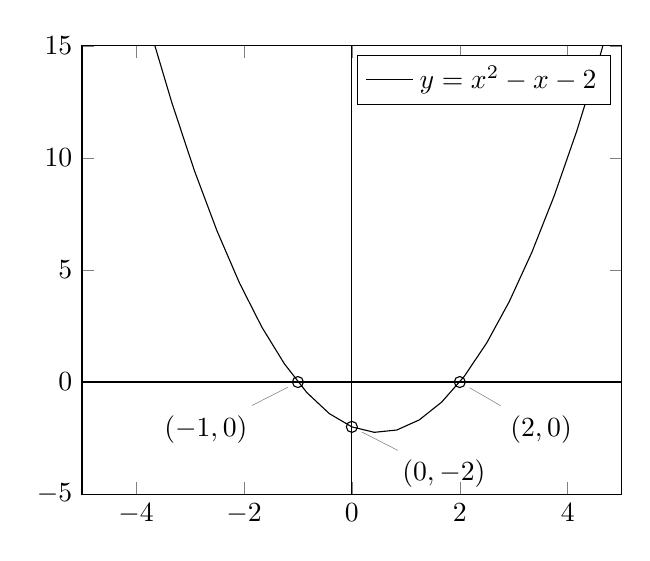
\begin{tikzpicture}
		\begin{axis}[
			xmin=-5, xmax=5,
    		ymin=-5, ymax=15,
		]
			\addplot[] {x^2 - x - 2};
			\addplot[only marks,mark=o] coordinates{(0,-2)} node[pin=-30:{$(0,-2)$}]{};
			\addplot[only marks,mark=o] coordinates{(-1,0)} node[pin=-150:{$(-1,0)$}]{};
			\addplot[only marks,mark=o] coordinates{(2,0)} node[pin=-30:{$(2,0)$}]{};
			\legend{$y=x^2 - x - 2$}
			\draw[-] (-8,0)--(8,0);
			\draw[-] (0,-25)--(0,15);		\end{axis}
	\end{tikzpicture}
\end{center}
\subsubsection{Sketching Parabolas from Completed Square Form}
To sketch a parabola from the completed square form we need to find 2 points: the y intercept (where $x=0$) and the turning point
(where $y$ is at its lowest value).
\\
Given a quadratic in the form $a(x+b)^2+c$ the turning point can be expressed as $(-b, c)$. This works because changing the
value of $b$ translates the graph on the $x$ axis and changing the value of $c$ translates the graph on the $y$ axis as show
below.
\\
For example, given the quadratic $(x + 2)^2 + 1$, the turning point is $(-3, 4)$ as shown on the graph below:

\begin{center}
	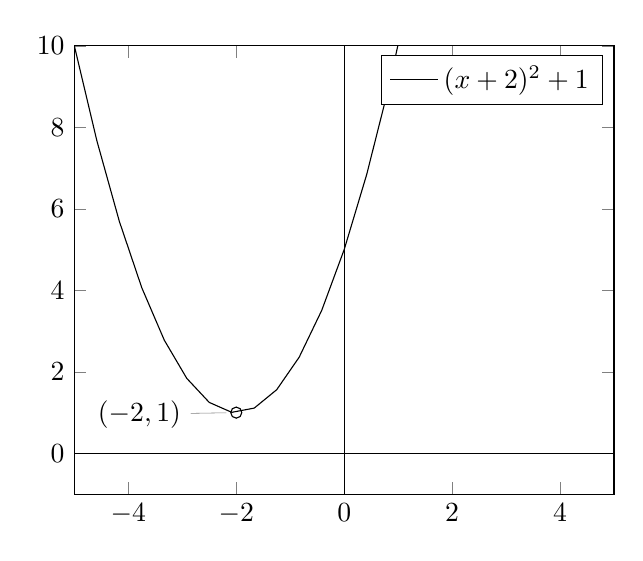
\begin{tikzpicture}
		\begin{axis}[
			xmin=-5, xmax=5,
    		ymin=-1, ymax=10,
		]
			\addplot[] {(x + 2)^2 + 1};
			\addplot[only marks,mark=o] coordinates{(-2,1)} node[pin=182:{$(-2,1)$}]{};
			\legend{$(x + 2)^2 + 1$}
			\draw[-] (-8,0)--(8,0);
			\draw[-] (0,-25)--(0,15);
		\end{axis}
	\end{tikzpicture}
\end{center}
To finish our sketch we need to find the $y$ intercept. To start we just replace $x$ with $0$ as were looking for the
point where $x=0$.
\\
For our previous example it would be as follows:

\begin{equation}
	y = (0 + 2)^2 + 1
\end{equation}
We then evaluate the right hand side of the equation to get our $y$ value:
\begin{equation}
	y = (0 + 2)^2 + 1 = (2)^2 + 1 = 4 + 1 = 5
\end{equation}
We can then use this information to plot our y intercept, $(0, 5)$, so we can sketch our graph.

\begin{center}
	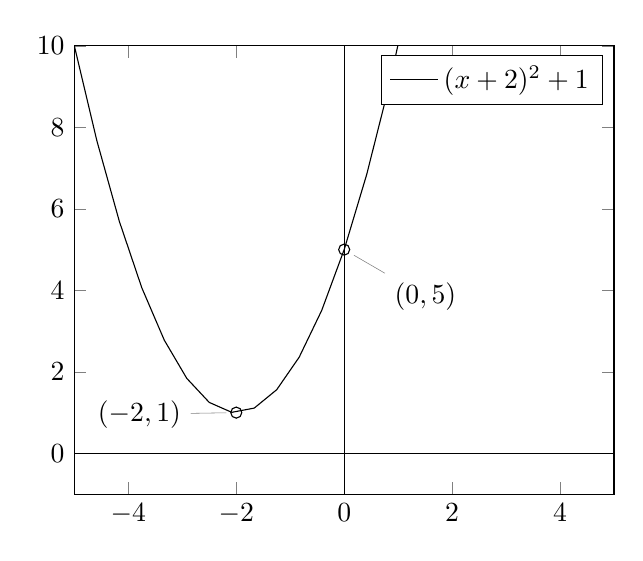
\begin{tikzpicture}
		\begin{axis}[
			xmin=-5, xmax=5,
    		ymin=-1, ymax=10,
		]
			\addplot[] {(x + 2)^2 + 1};
			\addplot[only marks,mark=o] coordinates{(-2,1)} node[pin=182:{$(-2,1)$}]{};
			\addplot[only marks,mark=o] coordinates{(0,5)} node[pin=-30:{$(0,5)$}]{};
			\legend{$(x + 2)^2 + 1$}
			\draw[-] (-8,0)--(8,0);
			\draw[-] (0,-25)--(0,15);
		\end{axis}
	\end{tikzpicture}
\end{center}
\break
\section{Surds}
Surds are the combination of a coefficient and a root in the form $a\sqrt{b}$ that can be used to 
represent a subset of irrational numbers.

\subsection{Simplifying Surds}

\begin{equation}
	\label{simple_equation}
	\sqrt{a} \times \sqrt{a} = a
\end{equation}
\begin{equation}
	\label{simple_equation}
	\sqrt{a} \times \sqrt{b} = \sqrt{ab}
\end{equation}
\begin{equation}
	\label{simple_equation}
	\frac{\sqrt{a}}{\sqrt{b}} = \sqrt{\frac{a}{b}}
\end{equation}

\subsection{Adding and subtracting surds}

\begin{equation}
	\label{bad_add}
	\sqrt{a} + \sqrt{b} \ne \sqrt{a + b}
\end{equation}

\begin{equation}
	\label{simple_surd_add}
	a\sqrt{c} + b\sqrt{c} = (a + b)\sqrt{c}
\end{equation}

\begin{equation}
	\label{surd_add}
	a\sqrt{c \times e} + b\sqrt{c \times d} = a\sqrt{c} \times \sqrt{e} + a\sqrt{c} \times \sqrt{d}
	 = (a\sqrt{e} + b\sqrt{d})\sqrt{c}
\end{equation}
\end{document}
